\documentclass[10pt,a4paper]{article}
\usepackage[utf8]{inputenc}
\usepackage[russian]{babel}
\usepackage[OT1]{fontenc}
\usepackage{amsmath}
\usepackage{amsfonts}
\usepackage{amssymb}
\usepackage{amsthm}
\usepackage{makeidx}
\usepackage{graphicx}
\usepackage{tikz}

\usepackage{graphicx}
\usepackage{caption}
\usepackage{subcaption}

\usepackage{float}
\floatstyle{boxed}
\restylefloat{figure}

\author{Максим Борисяк}
\title{Дипломная работа}
\makeindex

\newtheorem{defen}{Определение}
\newtheorem{example}{Пример}
\newtheorem{theorem}{Теорема}
%\newtheorem{proof}{Доказательство}

\newcommand{\stock}{\text{STOCK}}
\newcommand{\source}{\text{SOURCE}}
\newcommand{\initial}{\text{INITIAL}}
\newcommand{\nontrivial}{\text{NON-TRIVIAL}}
\newcommand{\map}{\text{MAP}}

\newcommand{\FA}{F\!A}

%\textheight = 720pt
%\textwidth = 500pt

%\hoffset = -25mm
%\voffset = -30mm

\makeindex

\begin{document}

\maketitle

\section{Введение}
В последние годы во многих областях науки, таких как, например, бионформатика или эксперементальная физика,
требуется обрабатывать все большее и большее количество данных.
В качестве примера можно привести Большой Адронный Коллайдер (БАК). 
В результате одного эксперимента поток 'сырых' данных с детектора \textit{ALICE} может превышать 1 гигабайт в секунду \textbf{[???]}.

Для обработки больших объемов данных используются распределенные вычислительные системы, мощности которых могут достигать пентафлопов.
Так для обработки данных БАК используется сложная распределенная система \textit{LHC Computing Grid}.
Такие мощности достигаются за счет громадного количества вычислительных узлов. Например, суперкомпьтер Sequoia мощностью более 1 пентафлопа
имеет более миллиона ядер \textbf{[???]}.

Однако с ростом объемов данных, и, как следствие, с ростом необходимых вычислительных ресурсов растет сложность задач эффективной обработки.
Известно, что принципы, лежащие в основе эффективных алгоритмов, могут существенно усложняться при переходе к параллельным вычислениям
и даже при изменении изменении масштабов вычислительных систем.

Другой проблемой становится сложность создания самих распределенных алгоритмов,
так как многие из них теряют наглядность из-за реализации большого количества технических аспектов, которые необходимо учитывать при их разработке.
Более того, некоторые распределенные системы не имеют четких границ, так как задействованные в ней участники могут постоянно меняться,
что дополнительно усложняет контроль за вычислениями.
Так для ускорения обработки результатов БАК был задействован проект \textit{LHC@home}, помочь которому мог любой желающий путем предоставления части
вычислительной мощности собственного компьютера.

Одним из решений описанных выше проблем стала концепция \textit{потоков данных} (\textit{dataflow}).
Под потоком данных обычно понимают модель представления алгоритмов.
Вычислительный процесс в такой концепции, обычно, представляет из себя следующие элементы:
\begin{itemize}
  \item набор атомарных исполнителей-функций, реализованный вне концепции потоков данных, например, в виде программ или динамических библиотек;
  \item описание зависимостей по данным между исполнителями --- результат одного исполнителя передается на вход другому;
  \item описание стратегии поведения потока данных.
\end{itemize}

Системы для построения и запуска потоков данных называются WFMS (WorkFlow Managment System)


\subsection{Мотивация}
Мотивация

\subsection{Обзор существующих система построения и запуска потоков данных}

\subsection{Неформальное описание модели}

\subsection{Базовые понятия и определения \textbf{*** Need review ***}}
В данном разделе будут введены базовые понятия, используемые в данной работе, в том числе,
понятия атомарного блока, составного блока, потока данных, автомата Мили соответствующего блоку и так далее.

Основной единицей потока данных является атомарный блок.
\begin{defen}
  \textbf{Шаблоном атомарного блока} $s$ назовем кортеж имеющий два не пересекающихся набора портов: \textit{входной} и \textit{выходной}.
  $s = (\FA, I, O)$, где:
  \begin{itemize}
    \item $I = \{b^I_i \vert i = \overline{1, N_I}, N_I \in \mathbb{N}\}$ --- конечное множество уникальных входных портов;
    \item $O = \{b^O_i \vert i = \overline{1, N_O}, N_O \in \mathbb{N}\}$ --- конечное множество уникальных выходных портов;
    \item $\FA$ --- конечный автомат Мили, смысл и структура которого будет обсуждаться в дальнейшем.
  \end{itemize}
\end{defen}
Сразу заметим, что не любая тройка $(\FA, I, O)$ является шаблоном атомарного блока, так как $\FA$ должен
соответствовать множествам $I$ и $O$.

Стоит отметить, что природа множеств $O$ и $I$ совершенно не важна, например, они могут быть просто множеством чисел: $I, O = \{i \in \overline{1, \dots, N_{I, O}}\}$,
на практике часто используют строки для именования портов, так как порты могут существенно различаться по смыслу, а их именование помогает избежать путаницы.
Последний подход используется в рисунках.

\begin{defen}
  \textbf{Атомарным блоком} $b = (id, s, state)$, где:
  \begin{itemize}
    \item $id$ --- уникальный для всех блоков идентификатор;
    \item $s$ --- шаблон атомарного блока;
    \item $state \in S$, где $S$ множество состояний $\FA_s$ --- текущее состояние атомарного блока.
  \end{itemize}
\end{defen}

Идентификатор $id$ введен из-за следующих соображений: в потоке данных некие блоки могут описываться одним и тем же шаблоном, находиться в одном и том же состоянии,
но все равно будут являться различными блоками, в частности, могут перейти в различные состояния в следующие моменты времени либо могут иметь в потоке данных разный смысл и,
соответственно, иметь различные соединения с другими блоками.

В реальных системах для построения и запуска потока данных шаблон атомарного блока представляется в виде подпрограммы или модуля
(функции, класса некого объектно-ориентированного языка программирования, динамической библиотеки), который используя данные некого набора своих входных портов,
вычисляет и записывает данные в свои выходные порты. В таком случае, атомарный блок представляется в виде набора внутренних переменных,
либо (что тоже самое) в виде экземпляра класса объектно-ориентированного языка программирования соответствующего шаблону.
В такой интерпретации некую вычислимую функцию $f(x_1, x_2, \dots, x_n)$ можно представить в виде шаблона блока $b_f$
с входными портами $x_1, x_2, \dots, x_n$ и одним выходным портом $F$, который при получении данных со всех входных портов
выписывает значения функции $f(x_1, x_2, \dots, x_n)$ в порт $F$.

На рисунке \ref{map} схематично изображен шаблон блока \textit{Loop}, для которого $inputs(Loop) = \{xs, f\}$, $outputs(Loop) = \{fs, x\}$.

\begin{figure}[H]
  \centering

  \begin{subfigure}[b]{0.2\textwidth}
    \centering
    \includegraphics[width=\textwidth]{map_cg.pdf}
    \caption{Схема шаблона \textit{Loop}}
    \label{map:connection}
  \end{subfigure}
  ~
  \begin{subfigure}[b]{0.7\textwidth}
    \centering
    \includegraphics[width=\textwidth]{map_fa.pdf}
    \caption{Автомат Мили шаблона \textit{Loop}}
    \label{map:fa}
  \end{subfigure}
  
  \caption{Схематичное изображение шаблона блока \textit{Loop} (a) и соответствующего ему конечного автомата Мили (b).}
  \label{map}
\end{figure}

Основной структурой для построения схемы потока данных является составной блок.

\begin{defen}
 \textbf{Шаблоном составного блока} будем называть кортеж $c = (B, E, I, O)$, где:
 \begin{itemize}
    \item $B$ - конечное множество блоков (сразу заметим, что блоком может являться и составной блок, определенный ниже).
    \item $E$ - множество ребер вида $e_b = (b_1, b^O_{1}, b_2, b^I_{2})$, $b_1, b_2 \in B$, $b^O_{1} \in outputs(b_1), b^I_{2} \in inputs(b)$,
                либо вида $e_I = (c^I, b, b^I)$, $e_O = (b, b^O, c^O)$, где $b \in B$, $b^I \in inputs(b)$, $b^O \in outputs(b)$, $c^O \in O$, $c^I \in I$.
                Множества ребер $e_b$ будем обозначать как $E^B$, $e_I$ и $e_O$ как $E^I$ и $E^O$ соответственно.
    \item $I$, $O$ - наборы входных и выходных портов (по аналогии с атомарным блоком).
  \end{itemize}
\end{defen}

В дальнейшем в выражениях вида $I_c$ или $O_c$ нижний индекс будет указывать на схему блока, которому принажлежат эти множества.

Для анализа внутренней структуры удобно рассматривать иное представление шаблона составного блока $c$, добавляя фиктивные блоки $\stock$, $I_{\stock} = O_{\stock} = O_c$,
  и $\source$, $I_{\source} = O_{\source} = I_c$:
$$\hat{E}^I = \{(\source, \source^O, b, b^I) \vert (\source^O, b, b^I) \in E^I\}$$
$$\hat{E}^O = \{ (b, b^O, \stock, \stock^I) \vert (b, b^O, \stock) \in E^O \}$$
$$\hat{c} = (B \cup \{\stock, \source\}, E^B \cup \hat{E}^I \cup \hat{E}^O)$$
В этом случае шаблон составного блока $\hat{c}$ описывается графом с ребрами вида $(u, u^O, v, v^I)$,
а входными и выходными портами всего шаблона считаются входные и выходные порты блоков $\source$ и $\stock$.
На рисунке \ref{example} изображен примеры шаблонов составных блоков во втрой интерпретации.

\begin{defen}
  \textbf{Составным блоком} будем называть $b = (id, c = (B, E, I, O), state)$, где
  \begin{itemize}
    \item $id$ --- уникальный идентификатор;
    \item $c$ --- шаблон составного блока;
    \item $state \in \Sigma \times 2^E = \prod S(B) \times 2^E \times 2^B$ - текущие состояние составного блока, включающее
          состояние каждого блока (подпространство $\Sigma = \prod S(B)$), активную волну ($\omega \in \Omega = 2^E$) и
          множество активных блоков ($\vartheta \in \Theta = 2^B$), смысл которых будет пояснен позже.
  \end{itemize}
\end{defen}

\begin{figure}[H]
  \centering
  \begin{subfigure}[b]{0.3\textwidth}
    \centering
    \includegraphics[width=\textwidth]{example_cg.pdf}
    \caption{Шаблон составного блока}
    \label{example:composite}
  \end{subfigure}
  ~
  \begin{subfigure}[b]{1.0\textwidth}
    \centering
    \includegraphics[width=\textwidth]{cc_cg.pdf}
    \caption{Шаблон супер-составного блока. Внутри рамки показана структура шаблона внутреннего блока.}
    \label{example:supercomposite}
  \end{subfigure}
  
  \caption{ Примеры графов составного и супер-составного блока.}
  \label{example}
\end{figure}

Заметим, что составной блок (в исходной интерпретации) внешне не отличим от атомарного блока.
Поэтому под понятием блока мы будем подразумевать либо атомарный блок, либо составной блок,
различая их только в том случае, когда речь заходит о их внутреннем строении. Составной блок может включать в себя другие составные блоки.
На рисунке \ref{example:supercomposite} показан пример составного блока, включающего другой составной блок, иными словами супер-составного блока.
На практике свойство вложенности реализует принцип модульности программ --- модулем в нашем случае будет шаблон составного блока.
Бессмысленно рассматривать случаи, в которых структура составного блока бесконечна в глубину, например,
в случае когда шаблон составного блок содержит содержит блок того же шаблона. Поэтому в дальнейшем, мы будем рассматривать только составные блоки конечной глубины.

Заметим, что составным блоком можно описать любую программу, имея в распоряжении необходимые примитивы --- шаблоны атомарных блоков,
реализующие Тьюринг-полную систему операций. Доказательства этого факта выходит за задачи данной работы и может быть найдено, например, в работе \textbf{[???]}.
Из-за достаточной выразительности составного блока, схему потока данных мы определим просто как схему некого составного блока.

Теперь неформально поясним схему работы составного блока и смысл его структуры.
В общепринятых определениях потока данных ребра графа шаблона составного блока обозначают зависимость по данным, то есть ребро $e = (u, u^O, v, v^I)$ представляет собой
\textit{FIFO}-канал соединения между портами блоков и
можно словесно интерпретировать следующим образом: блок $v$ в качестве данных из входного порта $v^I$ должен использовать данные выходного порта $u^O$ блока $u$ при их наличии.
Блок $u$ после завершения своей работы может "испустить данные по порту $u^O$", которые мгновенно "переносятся" на все ребра из $u^O$ блока $u$,
если эти ребра свободны.
Когда блоку $v$ требуются данные из порта $v^I$, данные с ребра $e$ мгновенно "переносятся" в соответствующий порт блока. В этом и есть смысле подпространства $\Omega = 2^E$
в определении состояния составного блока --- \textit{активной волной} $\omega$ мы назовем множество ребер, которые содержат на данный момент данные.

Однако такая схема работы составного блока порождает множество неопределенностей в работе некоторых составных блоков, например, неопределенность выбора ребра для "поглощения" данных из определенного порта (состояние гонки).
Неопределенности подобного рода мы будем рассматривать как ошибки, обнаружению которых посвящена часть данной работы. Такого рода неодназначности, особенно в реальных системах,
то есть в условиях неопределенного времени вычислений блоков и их параллельного выполнения, может привести к совершенно иному ходу потока данных, нежели было задумано автором потока данных.
Поэтому наличие подобного рода неопределенностей (состояний гонки) говорит скорее о неправильном построении схемы потока данных, чем о некой задумке автора потока данных.
Более подробно и строго об неоднозначностях в поведении потока данных будет идти речь ниже.
Стоит заметить, что подобного рода неоднозначности возникают и в процессе определения сетей процессов Кана,
которые решаются наложением условий на правила поглощения и испускания, а также на класс функции процесса.
Мы же пойдем другим путем, накладывая ограничения лишь на граф шаблона потока данных, оставляя подпрограммы и правила поглощения каждого шаблона блока без ограничений.
В нашем случае правила поглощения состоят в том, что формально блок может поглотить любые доступные данные из любых портов по любым ребрам,
но будем расценивать любые возможные неоднозначности как ошибку построения потока данных.

Выше были рассмотрены определения и термины, которые с той или иной точностью присутствуют практически во всех моделях потока данных.
В данной работе мы абстрагируемся от данных, а значит нас интересуют только возможные зависимости наборов входных портов от набора выходных портов,
иными словами только качественное поведение блоков. Оказывается, конечный автомат Мили хорошо подходит для описания качественного поведения блоков.
Заметим, что в данной работе используется не стандартное определение автомата Мили, а его недетерминированные аналог.
Дадим теперь строгое определение конечного автомата Мили.

\begin{defen}
  \textbf{Конечный автомат Мили} --- кортеж $\FA = (S, s_0, \Sigma, \Lambda, E)$, где:
  \begin{itemize}
    \item $S$ --- конечное множество состояний;
    \item $s_0 \in S$ --- начальное состояние;
    \item $\Sigma$ --- входной алфавит;
    \item $\Lambda$ -- выходной алфавит;
    \item $E \subseteq S \times \Sigma \times \Lambda \times S$ --- отношение возможных переходов.
  \end{itemize}
\end{defen}

Для удобства будем рассматривать функцию конечного автомата Мили $\FA = (S, \cdot, \Sigma, \Lambda, E)$:
$\FA(p, \sigma) = \{(\lambda, q, \sigma') \vert (p, \sigma', \lambda, q) \in E, \sigma' \subseteq \sigma\}$.
Стоит обратить внимание на нестандартную форму данной функции. Далее символами в алфавитах $\Sigma$ и $\Lambda$ будут множества, поэтому функция по текущему состоянию и входному множеству возвращает множество троек вида:
выходной символ-множество, новое состояние и поглощенное множество.

Конечный автомат Мили выполняет преобразование последовательности входных символов из алфавита $\Sigma$ в последовательность символов в алфавите $\Lambda$.
Вернемся теперь к определению шаблона атомарного блока. В данной работе мы абстрагируемся от конкретного алгоритма преобразования входных данных в выходные
и преобразования внутреннего состояния блока. Вместо этого мы будем описывать лишь качественное поведение алгоритма автоматом Мили $\FA$, в котором входной алфавит
$\Sigma = 2^I \setminus \varnothing$ (запрещается запуск по пустому набору входных портов),
а выходной алфавит $\Lambda = 2^O$, иными словами ребро $e = (u, is, os, v)$ автомата $\FA$ описывает возможный переход из состояния $u$ в состояние $v$,
при считывании данных из портов $is$ и выписывании данных в порты $os$ (именно поэтому функция $\FA$ имеет странный на первый взгляд вид).
На практике подпрограмма реализующая логику атомарного блока может иметь значительное количество внутренних состояний,
однако, для наших целей важны лишь группы таких внутренних состояний, которые описывают возможное поведение на определенном наборе данных из входных портов.
Более того практически во всех системах построения и запуска потока данных подпрограмма описывающая блок имеет детерминированное поведение.
Неизбежный недетерминизм в автомате Мили, описывающий блок, возникает из-за исключения из рассмотрения самих данных,
так как при разных значениях на одном и том же наборе портов из одного состояния, блок может перейти в различные конечные состояние,
даже выписав при этом данные в один и тот же набор портов.

\begin{example}
  На рисунке \ref{map:fa} изображен автомат Мили для шаблона атомарного блока $Loop$, описывающего цикл. Поясним эту схему.
  Изначально блок с шаблоном $Loop$ находиться в состоянии \textit{initial}.
  Далее он может считать из порта \textit{xs} начальные параметры цикла (например, некую коллекцию данных).
  Если условие выхода из цикла изначально выполнено (например, пустая коллекция), то блок переходит в прежнее состояние выписав в порт \textit{fs}.
  Иначе, блок отправляет данные по порту \textit{x} переходя в состояние \textit{non\_trivial}. В состоянии \textit{non\_trivial} блок имеет не тривиальное внутреннее состояние,
  например, остаток коллекции. В этот состоянии блок ожидает поступление преобразованных некой внешней функцией данных на порт \textit{f}.
  И в этом случае существует два варианта перехода, в зависимости от выполнения условия выхода из цикла:
  $(non\_trivial, \{f\}, \{x\}, non\_trivial)$ и $(non\_trivial, \{f\}, \{fs\}, trivial)$ для случаев продолжения цикла и выхода из него соответственно.
\end{example}

Конечный автомат Мили может быть также определен для составного блока. Единственное отличие от автомата Мили для атомарного блока состоит в том, что
зная все автоматы внутренних блоков, можно вычислить автомат составного блока как будет показано ниже.

\subsubsection{Алгоритм работы потока данных \textbf{***Need review***}}
Теперь опишем алгоритм вычисления потока данных, представленного в виде составного блока $c$ со схемой
$C = (\hat{B}_c = B_c \cup \{\source, \stock\}, \hat{E}_c= E_c \cup E^I_c \cup E^O_c)$ в представлении графа.
Мы будем рассматривать вычисление потока данных в предположении,
что время работы блока может быть абсолютно любым (но конечным) при любых условиях, что полностью соответствует реальным потокам данных.
В таком случае нас прежде всего будет интересовать всевозможные поведения потока данных с точки зрения относительных расположений времен запуска и завершения любого блока.
Введем модельное время $t \in \mathbb{Z}_+$.
Каждое множество, связанное с состоянием системы в момент времени $t$, снабдим верхним индексом, например, $\omega^t \in \Omega_c$.

\begin{defen}
  Определим некоторые вспомогательные функции.
  \begin{eqnarray*}
    O_v(\omega) & = & \{v^O \vert (v, v^O, \cdot, \cdot) \in \omega\}, \\
    I_v(\omega) & = & \{v^I \vert (\cdot, \cdot, v, v^I) \in \omega\}, \\
    \Delta_{O, v} & = & \{(v, v^O, \cdot, \cdot) \in E_c \vert v^O \in O\}, \\
    \Delta_{I, v} (\omega) & = & \{\tilde \omega_{I, v} \subseteq \omega \}, \; \forall \tilde \omega_I \forall v^I \in I \exists ! e \in \omega_I: e = (\cdot, \cdot, v, v^I)
  \end{eqnarray*}
\end{defen}
Последняя функция возвращает множество вариантов поглощения по набору входных портов $I$ блока $v$.

\begin{defen}
  Фронтом $\Psi_c (\omega, s)$ активной волны $\omega = \{(u, u^O, v, v^I)\} \in \Omega_c$ в состоянии $(s = (s_{u_1}, s_{u_2}, \dots, s_{u_m}), \omega, \cdot)$
  назовем подмножество блоков $\Psi_c (\omega, s) \subseteq B_c$, такое что:
  $$\Psi_c (\omega, s) = \{ v \in B \vert \FA_v(s_v, I_v(\omega)) \neq \varnothing\}$$
\end{defen}
Иными словами, фронт активной волны в заданном состоянии --- множество блоков, которые могут быть запущенны на следующем шаге.

\begin{defen}
  Семейство $\pi^t_v \in E_v, \; \FA_v = (\cdot, \cdot, E_v, \cdot)$ показывает текущий переход, который совершает блок $v$ в момент времени $t$.
\end{defen}
Заметим, что значение $\pi^t_v$ имеет смысл только для работающих на шаге $t$ блоков.

\begin{defen}
  Условием излучения назовем $\zeta(\omega^t, \omega^O) \Leftrightarrow (\omega^O \cap \omega^t = \varnothing)$.
  Также определим семейства $\zeta^t_v$:
  $$\zeta^t = \{ v \in B_c \vert zeta(\omega^t, \omega^O_v) \}$$
  $$\omega^O_v = \{ e \in E_c \vert e = (v, v^O, \cdot, \cdot), v^O \in O^t_v \}, \; (\cdot, O^t_v, \cdot, \cdot) \in \pi^t_v$$
\end{defen}
Условие излучение звучит довольно просто: блок может излучить, если все ребра соединенные с выходным набором портов свободны.

Пусть $\phi^t \subseteq \vartheta^t$ --- множество блоков, которые закончат работу после шага $t$. Для любого времени это множество может быть произвольным подмножеством $\vartheta^t$.
Однако для любого семейства этих множеств должно выполняться условие конечной работы блока: $\forall t \forall b \in \theta^t \exists \tau > t: b \in \phi^{\tau}$.

Так же для удобства введем обозначение для любого множества $A_c$ блоков из $B_c$ --- $A_c(v) \Leftrightarrow v \in A_c, v \in B_c$.

Теперь выпишем алгоритм преобразования потока данных в виде условий на переходы каждого блока из одного множества в другое.
В каждый момент времени блок $v$ может находиться в одном из трех состояний (множеств): свободен ($v \in \xi^t$), работает($v \in \theta^t$), заблокирован($v \in \chi^t$).
Время работы блоков задается $\phi^t \subseteq \vartheta^t$ --- множеством блоков, которые закончат работу после шага $t$. Для любого времени это множество может быть произвольным подмножеством $\vartheta^t$. Однако для любого семейства этих множеств должно выполняться условие конечной работы блока: $\forall t \forall b \in \theta^t \exists \tau > t: b \in \phi^{\tau}$.
Эти состояние взяты из реальных систем запуска потоков данных и служат для интуитивного понимания модели. В дальнейшем, однако, мы избавимся от этих состояний.
Также введем семейства  --- переход автомата Мили блока, который совершает блок в текущий момент.

\begin{eqnarray}
  % Free and can not be launched => Free
  \xi^t(v) \wedge \neg \Psi_c(\omega^t, s^t)(v) & \Rightarrow &
    \begin{cases}
      \xi^{t + 1}(v), \\
      s^{t + 1}_v = s^t_v, \\
      \omega^t_{I, v} = \omega^t_{O, v} = \varnothing
    \end{cases} \label{freetofree} \\
    % Free and can be launched => Work
  \xi^t(v) \wedge \Psi_c(\omega^t, s^t)(v) \wedge v \neq \stock & \Rightarrow &
    \begin{cases}
      \theta^{t + 1}(v), \\
      (\cdot, \cdot, I^t_v) \in \FA_v(s^{t}_v, I_v(\omega^t)), \\
      \pi^{t + 1}_v \in \{ (s^t_v, I^t_v, \cdot, s^{t + 1}_v) \in E_v\}, \\
      \omega^t_{I, v} \in \Delta_{I^t_v, v}(\omega^t), \\
      \omega^t_{O, v} = \varnothing
    \end{cases} \label{freetostart}
\end{eqnarray}

\begin{eqnarray}
  % Work and will not finish => Work
  \theta^t(v) \wedge \neg \phi^t(v) & \Rightarrow &
   \begin{cases}
     \theta^{t + 1}(v), \\
     s^{t + 1}_v = s^t_v, \\
     \pi^{t + 1}_v = \pi^t_v, \\
     \omega^t_{I, v} = \omega^t_{O, v} = \varnothing
   \end{cases} \label{worktowork} \\
   % Work, will finish and can be finished => Free
  \theta^t(v) \wedge \phi^t(v) \wedge \zeta^t(v) & \Rightarrow &
    \begin{cases}
      \xi^{t + 1}(v), \\
      (s^t_v, \cdot, O^t_v, s^{t + 1}_v) = \pi^t_v, \\
      \omega^t_{O, v} = \Delta_{O^t_v, v}, \\
      \omega^t_{I, v} = \varnothing
    \end{cases} \label{worktofree}\\
  % Work, will finish and can not be finished => Blocked
  \theta^t(v) \wedge \phi^t(v) \wedge \neg \zeta^t(v) & \Rightarrow &
    \begin{cases}
      \chi^{t + 1}(v),\\
      \pi^{t + 1}_v = \pi^t_v, \\
      \omega^t_{O, v} = \omega^t_{I, v} = \varnothing
    \end{cases} \label{worktoblock}
\end{eqnarray}

\begin{eqnarray}
  % Blocked and can release data => Free
  \chi^t(v) \wedge \zeta^t(v) & \Rightarrow &
    \begin{cases}
      \xi^{t + 1}(v), \\
      (s^t_v, \cdot, O^t_v, s^{t + 1}_v) = \pi^t_v, \\
      \omega^t_{O, v} = \Delta_{O^t_v, v}, \\
      \omega^t_{I, v} = \varnothing
    \end{cases} \label{blocktofree} \\
  % Blocked and can not release data => Blocked
  \chi^t(v) \wedge \neg \zeta^t(v) & \Rightarrow &
    \begin{cases}
      \chi^{t + 1}(v), \\
      s^{t + 1}_v = s^t_v, \\
      \pi^{t + 1}_v = \pi^{t}_v, \\
      \omega^t_{O, v} = \omega^t_{I, v} = \varnothing
    \end{cases} \label{blocktoblock}
\end{eqnarray}

\begin{eqnarray}
  \omega^{t + 1} & = & \omega^t \setminus (\cup_{v \in B_c} \omega^t_{I, v}) \cup (\cup_{v \in B_c} \omega^t_{O, v}) \label{newomega}, \\
  s^{t + 1} & = & (s^t_{v_1}, \dots, s^t_{v_m}) \label{newstate}
\end{eqnarray}

\begin{figure}
    \centering
    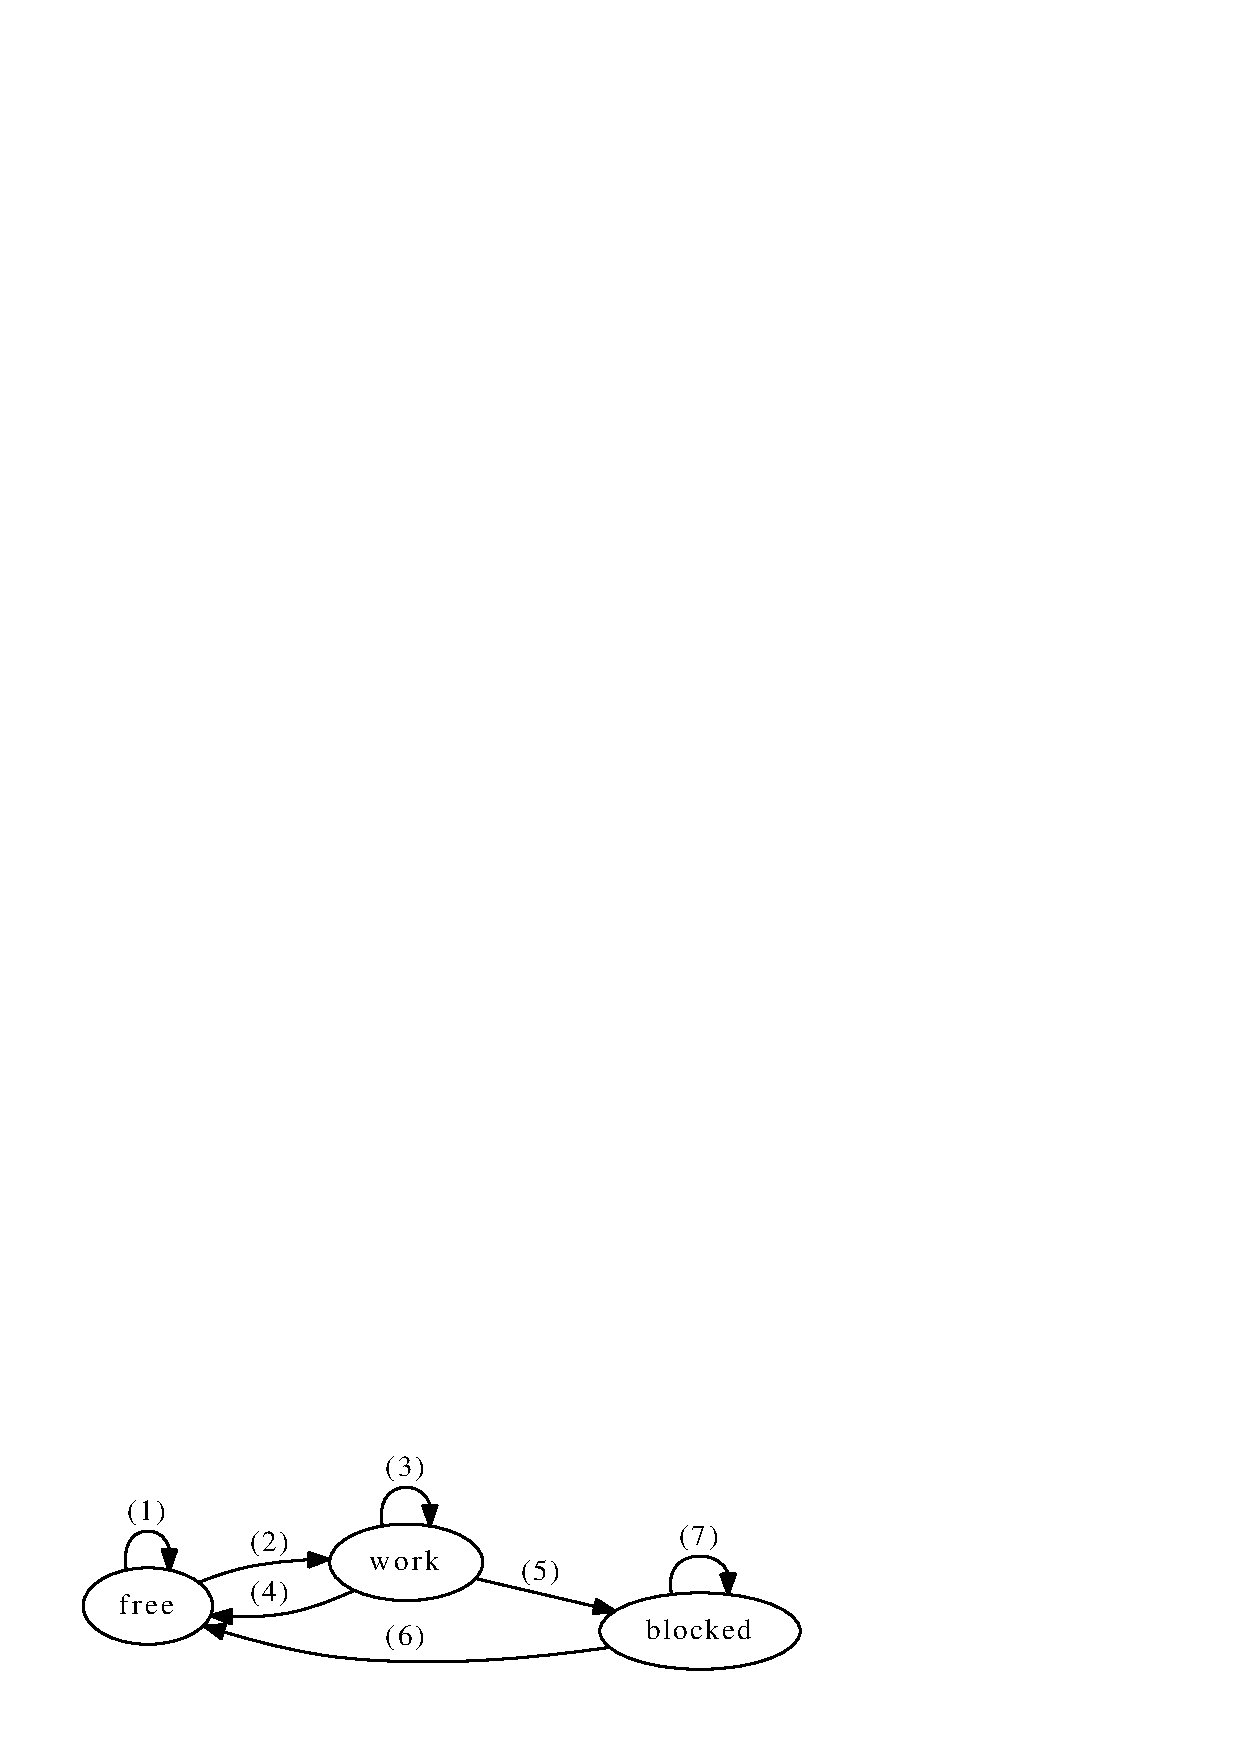
\includegraphics[width=\textwidth]{rules.pdf}
    \caption{Схема работы блока}
    \label{rules}
\end{figure}

Работу каждого блока можно схематично изобразить в виде автомата, см. рисунок \ref{rules}.

Поясним эти правила. Каждое правило \eqref{freetofree} --- \eqref{blocktoblock} описывает условие перехода в конечном автомате на рисунке \ref{rules}.

Правила \eqref{freetofree} и \eqref{freetostart} говорят о поведении свободного блока --- если блок может запуститься из его текущего состояния $s^t_v$
(то есть хватает данных на портах для какого-либо перехода), то он поглощает данные $\omega^t_{I, v}$ и
начинает некий переход $\pi^{t+1}_v$ из текущего состояния, иначе остается свободным дальше.

Тройка правил \eqref{worktowork}, \eqref{worktofree} и \eqref{worktoblock} описывают поведение работающего блока $v$. Если множество $\phi^t$ не содержит рассматриваемый блок,
он продолжает работу. Иначе, возможны два варианта: либо блок может завершиться и испустить данные $\zeta^t(v)$ (то есть ребра $\Delta_{O^t_v, v}$, связанные с
испускаемыми портами $O^t_v$, свободны), то блок благополучно завершает работу $\xi^{t + 1}(v)$ и испускает данные ($\omega^t_{O, v}$),
либо блок переходит в состояние блокировки до момента, когда требуемые ребра освободятся, которое описывается правилами \eqref{blocktofree} и \eqref{blocktoblock}.

Заметим, что мы специально различаем состояния блокировки и работы, хотя можно было бы считать, что заблокированный блок просто работает дополнительное время.
Состояние блокировки отличается тем, что блок в этом состоянии не требует вычислительных ресурсов, что будет важно в дальнейшем.

Заметим, что в правилах поведения потока данных сразу видны все неопределенности, о которых говорилось ранее --- перед запуском блока, определяется переход,
который будет совершать блок, вместе с набором поглощаемых портов и ребра с которых эти данные будут поглащены. Подробнее мы будем рассматривать эти неопределенности далее.

\subsubsection{Начало и завершение работы потока данных}
  Если рассматривать представление потока данных в виде графа, то начало и завершение потока данных связанно с дополнительными или 'фиктивными'
  блоками $\source$ и $\stock$: их задачи сформировать начальную и поглотить конечную активные волны, соответственно.
  Исходя из правил, можно записать начальные условия:
  \begin{eqnarray}
    \omega^0 & = & \varnothing, \\
    s^0_v & = & s_{0, v}, \forall v \in B_c, \\
    \theta^0 & = & \{\source\}, \\
    \xi^0 & = & B_c \setminus \{\source\}, \\
    \chi^0 & = & \varnothing, \\
    \omega^1 & \neq & \varnothing
  \end{eqnarray}
  
  Формирование начальной волны заложено в принципе работы блока $\source$.
  Так как блоки $\source$ и $\stock$ являются вспомогательными, то нет смысла рассматривать их автоматы Мили, так как атомат для блока $\source$ не может иметь ни одного перехода
  из-за отсутствия входных портов, а автомат для блока $\stock$ будет создавать дополнительные неопределенности при анализе потока данных.
  Будем считать, что работа этих блоков определяется следующим образом: $\source$ на первом шаге испускает некий непустой набор входных данных --- начальную активную волну;
  блок $\stock$ поглощает все данные на его портах, если никакие другие блоки больше не могут запуститься. Именно запуск блока $\stock$ мы будем считать завершением работы
  всего потока данных, иными словами, поток данных завершает работу на шаге $t = T_{end}$, если:
  \begin{equation}
    \theta^{T_{end}} = \varnothing \wedge \Psi_c(\omega^{T_end}, s^{T_end}) = \{\stock\}
    \label{end_of_workflow}
  \end{equation}
  Завершение работы потока данных связанно с понятием траектории запуска потока данных и более подробно будет рассмотренно ниже.

\section{Анализ модели}
\subsection{Построение конечного автомата Мили по программе блока \textbf{***Need review***}}
Введенная выше модель оперирует с упрощенными описаниями алгоритмов блоков --- каждый алгоритм заменяется на описывающий его качественное поведение автомат Мили.
Каждое состояние конечного автомата соответствует группам внутренних состояний алгоритма блока. Разбиение на группы можно производить с большой свободой.
Сразу же заметим, для дальнейшего анализа будет полезно выделить особое состояние конечного автомата Мили для блока --- начальное состояние (далее будет обозначаться словом $\initial$), соответствующее начальным значениям внутренних переменных. Это состояние обладает значительной особенностью, а именно, блок находящийся в нем, фактически
не занимает ресурсов памяти вычислительного узла, поэтому может быть просто перенесен на другой вычислительный узел без дополнительных затрат
на копирование внутреннего состояния с одного вычислительного узла на другой. Процедуры перемещения состояния алгоритма блока на другой
вычислительный узел играют важную роль в управлении запуском потока данных в распределенной среде (более подробно запуск потока данных в распределенной среде будет рассмотрен ниже), так как ожидающий данных блок будет заблокирован (или по, крайней мере, может быть дополнительно ограничен в вычислительных ресурсах),
если на вычислительном узле на момент поступления данных первому блоку выполняется алгоритм другого блока, но может быть инициализирован на свободном
(если таковые имеются) вычислительном узле, если блок находится в начальном состоянии.

Построение автомата Мили для алгоритма блока --- неодназначная задача, требующая понимания качественного поведения алгоритма, а значит участия человека. В данной работе подробно не рассматриваются алгоритмы (которые, по мнению автора, будут бесполезны на практике в силу огромных вычислительных затрат) и методики построения атоматов Мили для алгоритмов блоков. Ограничемся лишь рассмотрение показательного примера с шаблоном блока \textit{For-Loop}. В зависимости от реализации, блок \textit{For-Loop} принимает на вход данные о количестве необходимых операций, для опреденности будем рассматривать шаблон блока, реализующий аналог функции \textit{map} популярной в функциональных языках программирования,
которая поэлементно применяет переданную ей в качестве аргумента функцию к списку значений и выдает список результатов. Типичный пример составного блока с блоком шаблона $For-Loop$ показан на рисунке \ref{example:composite} (сам блок шаблона \textit{For-Loop} именуется \textit{map}), а автомат Мили шаблона блока \textit{For-Loop}
показан на рисунке \ref{map:fa}. Сам блок шаблона \textit{For-Loop} требует внешнего блока-функции, который подключен к портам \textit{x} и \textit{f}.
Между вызовами (то есть испусканием очередного элемента списка) блока-функции, блок шаблона \textit{For-Loop} имеет внутреннее состояние, в котором хранит, как минимум,
не обработанную часть списка и частичный результат преобразования. Поэтому в конечном автомате Мили шаблона блока \textit{For-Loop} имеются два состояния:
\textit{initial} --- начальное состояние ожидания данных, \textit{non\_trivial} --- состояние, в котором результирующий список находится в стадии формирования.

\begin{figure}
    \centering
    \includegraphics[width=\textwidth]{map_extra_fa.pdf}
    \caption{Избыточный конечный автомат Мили для шаблона блока \textit{For-Loop}}
    \label{map:extra_fa}
\end{figure}

Фактически, для любого алгоритма можно построить автомат Мили с не более, чем двумя состояниями: начальным (или тривиальным) и не тривиальным (с отличным от начального внутренним
состоянием) состояниями, однако, в некоторых случаях автомат Мили будет вносить дополнительную неопределенность в поведение блока, не связанную с неопределенностью
входных данных при анализе. Возможен и обратный случай --- в предыдущем примере с шаблоном блока \textit{For-Loop} можно ввести отдельное состояние, отвечающее за списки длины 1.
В данном случае автомат Мили будет выглядеть, как показано на рисунке \ref{map:extra_fa}, дополнительное состояние именуется \textit{length\_1}. Это дополнительное состояние, конечно,
несет новую информацию о текущем состоянии блока, но она абсолютно бесполезно для анализа схемы потока данных.

\subsection{Эквивалентность траекторий запуска потока данных \textbf{***Need review***}}
  Рассмотрим подробнее правила работы потока данных. В правилах помимо неопределенностей в выборе вариантов поведения, присутствует множество $\phi^t$, задаваемое извне.
  Фактически это множество определяет время работы каждого запущенного блока и введено для возможности описания любой возможной конфигурации времен работы алгоритмов блоков.
  Однако при анализе потока данных эти времена неизвестны и здесь не будут рассматриваться их оценки. Для анализа большее значения играет не сами времена работы блоков, а
  зависимости типа "запуск блока $A$ был вызван завершением работы блоков $B_1, B_2, \dots, B_l$".
  В дальнейшем, для выяснения всевозможных поведений потока данных в терминах этих зависимостей,
  мы будем эмулировать запуск потока данных по правилам \eqref{freetofree}-\eqref{newstate}, и, в частности, положим времена работы всех блоков равными единице.
  Модельное время в данном случае отражает лишь один из возможных случаев запуска потока данных и служит только для удобства понимания.
  Вначале определим понятие траектории запуска потока данных и введем на множестве траекторий запуска отношение эквивалентности.
  
  \begin{defen}
    Траекторию запуска потока данных $\Lambda = \{\Lambda^t\}_{t=0}^{\infty}$ мы определим как семейство всех множеств упомянутых в
    правилах работы потока данных \eqref{freetofree}-\eqref{newstate} и описывающих состояние потока данных,
    то есть $\Lambda^t = (\omega^t, \{\omega^t_{I, v} \vert v \in B_c\}, \{\omega^t_{O, v} \vert v \in B_c\}, \pi^t, s^t, \xi^t, \theta^t, \chi^t$.
  \end{defen}
  
  Введем также определения конечной и успешной траекторий и времени работы потока данных на этой траектории.
  \begin{defen}
    Траектория запуска потока данных $\Lambda = \{\Lambda^t\}_{t=0}^{\infty}$ называется конечной, если
    $\exists T_{end}: \forall t \geq T_{end}: \theta^t = \varnothing$. Минимальное $T_{end}$ называется временем работы потока данных.
    \label{def:trajectory_finite}
  \end{defen}
  
  \begin{defen}
    Траектория запуска потока данных $\Lambda = \{\Lambda^t\}_{t=0}^{\infty}$ называется успешной, если
    $\exists T_{end}: \forall t \geq T_{end} : \xi^t = B_c \wedge \omega^t = \varnothing$.
    \label{def:trajectory_success}
  \end{defen}
  
  Понятно, что минимальные $T_{end}$ из определений \ref{def:trajectory_finite} и \ref{def:trajectory_success} совпадают (если оба существуют), и более того, равны
  (с точностью до времени работы блока $\stock$, которое, для удобства положим равным $0$) $T_{end}$ в \eqref{end_of_workflow}, так как при отсутствии работающих
  блоков фронт активной волны $\omega^t$ не может меняться (в силу правила работы потока данных \eqref{newomega}),
  а значит правило \eqref{blocktofree} не может быть выполнено для заблокированных блоков, так как оно полностью определяется фронтом активной волны.
  В дальнейшем мы будем предполагать, что все траектории рассматриваемого потока данных являются конечными.
  
  Множества $\pi^t_v$, $\omega^t_{I, v}$ и $\omega^t_{O, v}$ полностью описывают отношение эквивалентности между траекториями.
  \begin{defen}
    Для каждой конечной траектории запуска множества $\pi^t_v$, $I^t_v$ пораждают граф причинности $G = (S, E)$.
    Для каждого блока пронумеруем все времена его запуска $t^n_v$. Тогда $G$ можно определить как:
    \begin{itemize}
      \item $S = \{ (v, n, \pi^{t^n_v}_v) \}$,\\
      \item из $s_1 = (v, \cdot, \pi_1)$ в $s_2 = (v, \cdot, \pi_2)$ есть ребро тогда и только тогда,
      когда часть поглощенной $\omega^t_{I, v}$ в результате перехода $\pi_2$ была испушена в результате перехода $\pi_1$;
      при этом ребро дополнительно помечается множеством соответствующих входных портов блока $v$.
    \end{itemize}
  \end{defen}
  
  Отображение $G_{\Lambda} = G(\Lambda)$ индуцирует классы эквивалентности траекторий запуска потока данных,
  иными словами $\Lambda_1 \sim \Lambda_2 \Leftrightarrow G(\Lambda_1) = G(\Lambda_2)$.
  Отметим, что данное отношение эквивалентности имеет смысл только для успешных траекторий, так как в нем не учитываются остаточные активные волны и заблокированные блоки.
  Наличие неуспешных траекторий потока данных мы будем рассматривать как ошибку проектирования схемы потока данных. Отметим, что это правило полностью соответствует практике.
  
  Каждый граф причинности качественно описывает запуск потока данных.
  
  \begin{example}
  \label{map_example}
  Рассмотрим один показательный пример нахождения графов причинности для потока данных, содержащего цикл (схема потока данных изображена на рисунке \ref{example:composite}).
  Для простоты, будем считать, что автомат Мили блока $f$ состоит из одного состояния и одного перехода $\pi_f = (\initial, \{x\}, \{f\}, \initial)$.  
  Наличие ребра из $s_1$ в $s_2$ в графе причинности будем обозначать как $s_1 \leadsto s_2$.
  
  Начальная вершина всех графов причинности --- $s_0 = (\source, 0, \pi_{\source})$. Далее возможны варианты: либо начальная вершина вызовет переход
  $\pi_{\map, 1} = (\initial, \{xs\}, \{fs\}, \initial)$ (то есть переход по пустому списку данных), либо $\pi_{\map, 2} = (\initial, \{xs\}, \{x\}, \nontrivial)$.
  Последний в свою очередь вызовет переход $\pi_f$, который, в свою очередь, может вызвать переходы
  $\pi_{\map, 3} = (\nontrivial, \{f\}, \{x\}, \nontrivial)$ и $\pi_{\map, 4} = (\nontrivial, \{f\}, \{xs\}, \initial)$, и так далее.
  Конечная вершина графа --- $s_{end} = (\stock, T_end, \pi_{\stock})$.
  Получаем семейство графов причинности:
  \begin{eqnarray*}
    s_0 & \leadsto & (\map, t_1, \pi_{\map, 1}) \leadsto s_{end}, \\
    s_0 & \leadsto & (\map, t_1, \pi_{\map, 2}) \leadsto (f, t_2, \pi_f) \leadsto (\map, t_3, \pi_{\map, 4}) \leadsto s_{end}, \\
    s_0 & \leadsto & (\map, t_1, \pi_{\map, 2}) \leadsto (f, t_2, \pi_f) \leadsto (\map, t_3, \pi_{\map, 3}) \leadsto \\
    & \leadsto & (f, t_4, \pi_f) \leadsto \dots \leadsto (\map, t_n, \pi_{\map, 4}) \leadsto s_{end}
  \end{eqnarray*}
  
  \end{example}
  
  Этот пример демонстрирует необходимость следующего предположения:
  \textit{будем считать, что любая циклическая зависимость конечна (то есть не будем рассматривать не конечные траектории, возникающие из-за этих зависимостей)}.
  
\subsection{Неопределенности в запуске потока данных \textbf{***Need review***}}
  Как было упомянуто выше, в анализе схемы потока данных неизбежно возникают два рода неопределенностей: первый вызван отсутствием знания входных данных при анализе схемы,
  неопределенности второго рода связанны с самой схемой потока данных, которая может допускать такие неоднозначности как, например, несколько вариантов поглощения данных.
  Неоднозначности первого рода неизбежны, и поэтому следует обрабатывать все варианты порожденные ими.
  Все эти неоднозначности второго рода возникают как следствие состояний гонки (race condition), которых традиционно стараются избегать,
  так как результат выполнения всего потока данных становиться зависим от времен работы блоков, которые, в свою очередь, могут зависеть от данных и
  параметров вычислительных узлов, что говорит скорее о неправильном построении схемы потока данных.
  
  Сформулируем теперь критерии неопределенностей первого и второго рода.
  
  Любые неопределенности связаны с правилом запуска потока данных \eqref{freetostart} --- правило запуска блока, что видно из правил работы потока данных, так как,
  только это правило содержит включения, вместо строгих равенств.
  \begin{defen}
    Будем говорить, что состояние $s$ автомата Мили $\FA_v = (S_v, \cdot, \cdot, \cdot, E_v)$ блока $v$ допускает неопределенность первого рода, тогда и только тогда, когда:
    $\exists I_v: \lvert \{e \in E_v \vert e = (s, I_v, \cdot, \cdot) \} \rvert > 1$, или иными словами, существует набор входных портов $I_v$, такой что, из состояния $s$ возможны
    несколько переходов по входным портам $I_v$.
  \end{defen}
  
  Например, в автомате Мили шаблона блока \textit{For-Loop} (рисунок \ref{map:fa}) каждое состояние допускает неопределенность первого рода.
  Причины возникновения этих неопределенностей были описанны выше.
 
  \begin{defen}
    Блок $v \in B_c$ в состоянии $\Lambda^t$ траектории запуска потока данных на шаге $t$ допускает неопределенность второго рода, если:
    $\lvert \omega^t_{I, v} \rvert > 1$, где $\omega^t_{I, v}$ определена в правиле \eqref{freetostart} и содержиться в кортеже $\Lambda^t$.
  \end{defen}
  
  \begin{defen}
    \textbf{Корректным потоком данных} будем называть поток данных, любая возможная траектория которого не допускает неопределенностей второго рода.
  \end{defen}
  
  Заметим, что по автомату Мили можно сразу предсказать возможные неопределенности второго рода, например, если автомат Мили содержит переходы
  $\pi = (s, I, \cdot, \cdot)$ и $\pi' = (s, I', \cdot, \cdot)$,
  где $I \subseteq I'$: в этом случае переход по $\pi'$ автоматически означает неопределенность второго рода,
  соответственно, наличие таких переходов автоматически означает неправильность построения автомата Мили или алгоритма блока.
  
  Введем вспомогательное определение набора последовательностей времен работы блоков.
  \begin{defen}
    Зафиксируем набор последовательностей времен работы $\tau = \{\{\tau^n_v\}^{\infty}_{n = 0} \vert v \in B_c\}$.
    Траектория $\Lambda$ согласуется с набором последовательностей времен запуска, если время работы $n$-го запуска блока $v$ $t^n_v = \tau^n_v$.
  \end{defen}
  
  \begin{theorem}
    В работе потока данных не существует других неопределенностей, кроме неопределенностей первого и второго рода, то есть,
    если зафиксировать набор последовательностей времен работы блоков $\tau$, то любое ветвление префиксного дерева траекторий, согласующихся с $\tau$,
    описывается только неопределенностями первого и второго рода.
  \end{theorem}
  \begin{proof}
    Доказательство напрямую следует из факта, что любые различия в траекториях запуска потока данных при фиксированных временах работы блоков определяются
    правилом \eqref{freetostart} работы потока данных.
  \end{proof}
  
  Среди неопределенностей второго рода следует выделить важный случай, уже упоминавшийся выше --- состояние гонки.
  
  \begin{defen}
    Поток данных допускает состояние гонки, если существует некая последовательность времен запуска $\tau$ и класс эквивалентности $\mathbb{K}$
    траекторий запуска потока данных, такие что траектории удовлетворяющие $\tau$ не лежат в классе $\mathbb{K}$.
  \end{defen}
  
  Поясним это определение. Из определения сразу же следует, что в отсутствии состояния гонки, каждый класс эквивалентности для любого набора последовательностей
  времен запуска содержит траекторию, согласующуюся с ней, что означает то,
  что результат не зависит от времен работы блоков (что соответствует классическим определениям).
  
\subsection{Волновой алгоритм}  
  Решение задачи нахождения классов эквивалентности траекторий запуска позволяет существенно упростить анализ потока данных, так как
  переход к графам причинности позволяет избавиться от модельного времени для корректных потоков данных.
  
  Однако, даже для корректного потока данных, классов эквивалентности может быть бесконечное количество. Это утверждение было проиллюстрированно в примере \ref{map_example}.
  Одним из возможных решений этой проблемы --- нахождение циклов и их замена на соответствующий составной блок. Однако, это не всегда удается, например,
  из-за того, что 'тело' цикла может иметь связи с самим блоком цикла. Однако, если замена циклов удалась, то поток данных будет преобразован к ацикличному графу,
  работу которого заметно проще анализировать. Однако в данной работе мы пойдем другим путем.
  
  Мы будем находить 

\subsection{Работа волнового алгоритма в графе переходов}



\end{document}